\documentclass[border=5pt]{standalone}
\usepackage{tikz}
\usepackage{amsmath}
\begin{document}
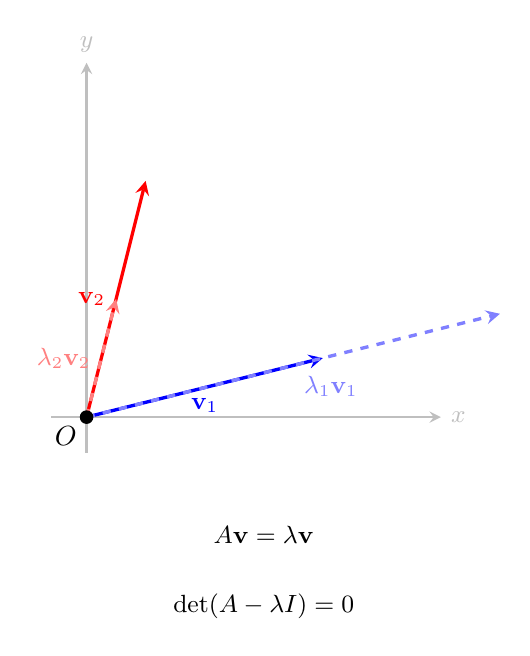
\begin{tikzpicture}[scale=1.5, >=stealth]
  % Eigenvectors: directions preserved under transformation

  % Axes
  \draw[->, thick, gray!50] (-0.3,0) -- (3,0) node[right, font=\small] {$x$};
  \draw[->, thick, gray!50] (0,-0.3) -- (0,3) node[above, font=\small] {$y$};

  % Eigenvector 1 (stretched)
  \draw[->, very thick, blue] (0,0) -- (2,0.5) node[midway, below, font=\small] {$\mathbf{v}_1$};
  \draw[->, very thick, blue!50, dashed] (0,0) -- (3.5,0.875) node[midway, below right, font=\small] {$\lambda_1\mathbf{v}_1$};

  % Eigenvector 2 (compressed)
  \draw[->, very thick, red] (0,0) -- (0.5,2) node[midway, left, font=\small] {$\mathbf{v}_2$};
  \draw[->, very thick, red!50, dashed] (0,0) -- (0.25,1) node[midway, left, font=\small] {$\lambda_2\mathbf{v}_2$};

  % Origin
  \filldraw[black] (0,0) circle (1.5pt) node[below left] {$O$};

  % Formula
  \node[font=\small] at (1.5, -1) {$A\mathbf{v} = \lambda\mathbf{v}$};
  \node[font=\small] at (1.5, -1.6) {$\det(A - \lambda I) = 0$};
\end{tikzpicture}
\end{document}
